\documentclass[12pt,letterpaper]{article}
\usepackage[utf8]{inputenc}
\usepackage[spanish]{babel}
\usepackage{graphicx}
\usepackage[hidelinks]{hyperref}
\usepackage{hyperref}
\usepackage[left=2cm,right=2cm,top=2.5cm,bottom=2cm]{geometry}
\usepackage{graphicx} % figuras
\usepackage{float} % para usar [H]
\usepackage{amsmath}
\usepackage{stackrel} 
\usepackage{multicol}
\usepackage{multirow}
\usepackage{fancyhdr}
\usepackage[usenames,dvipsnames,svgnames,table]{xcolor}
\usepackage[document]{ragged2e}
\usepackage{enumerate} % enumerados
\renewcommand{\labelitemi}{$-$}
\renewcommand{\labelitemii}{$\cdot$}

\begin{enumerate}
	\begin{titlepage}
		\begin{center}
			\begin{figure}[htb]
				\begin{center}
					
\includegraphics[width=3.5cm]{./img/upt}
				\end{center}
			\end{figure}
			\vspace*{0.15in}
			\begin{Large}
				\textbf{UNIVERSIDAD PRIVADA DE TACNA}\\
			\end{Large}
			\vspace*{0.15in}
			\begin{Large}
				\textbf{FACULTAD DE INGENIERIA} \\
			\end{Large}
			\vspace*{0.1in}
			\begin{Large}
				\textbf{Escuela Profesional de Ingeniería de Sistemas} \\
			\end{Large}
			\vspace*{0.3in}
			\begin{Large}
				\textbf{INFORME DE LABORATORIO N°01}\\
				\textbf{“Crear y consultar una tabla NoSQL”}\\
			\end{Large}
			\vspace*{0.2in}
			\begin{Large}
				\textbf{CURSO:} \\
			\end{Large}
			\vspace*{0.1in}
			\begin{large}
				Base de Datos II\\
			\end{large}
			\vspace*{0.2in}
			\begin{Large}
				\textbf{DOCENTE:} \\
			\end{Large}
			\vspace*{0.1in}
			\begin{large}
				Ing. Patrick Jose Cuadros Quiroga\\
			\end{large}
			\vspace*{0.3in}
			\begin{large}
				\textbf{ALUMNO:} \\
				\begin{flushleft}
					Risther Jaime Tarqui Montalico  		\hfill	(2017057469) \\
				\end{flushleft}
			\end{large}
			\vspace*{1.3in}
			\begin{large}
				Tacna - Perú\\
			\end{large}
			\vspace*{0.1in}
			\begin{large}
				2020\\
			\end{large}
		\end{center}
	\end{titlepage}
	\include{Secciones/articulo}
	\newpage
	
	\justify
	
	\begin{LARGE}
		\begin{center}
			\textbf{Crear y consultar una tabla NoSQL} \\
		\end{center}
	\end{LARGE}
	\section{OBJETIVO}
	\begin{itemize}
		\item crear una tabla simple, agregar datos, analizar y realizar consultas sobre los datos, eliminar datos y eliminar la tabla con la consola de DynamoDB.
	\end{itemize}
	
	\section{DESARROLLO}
	\item Abra la consola de administración de AWS para poder mantener abierta esta guía paso a paso. Cuando se cargue esta pantalla empiece a escribir DynamoDB en la barra de búsqueda y seleccione la opción para abrir la consola de DynamoDB.
		\begin{center}
		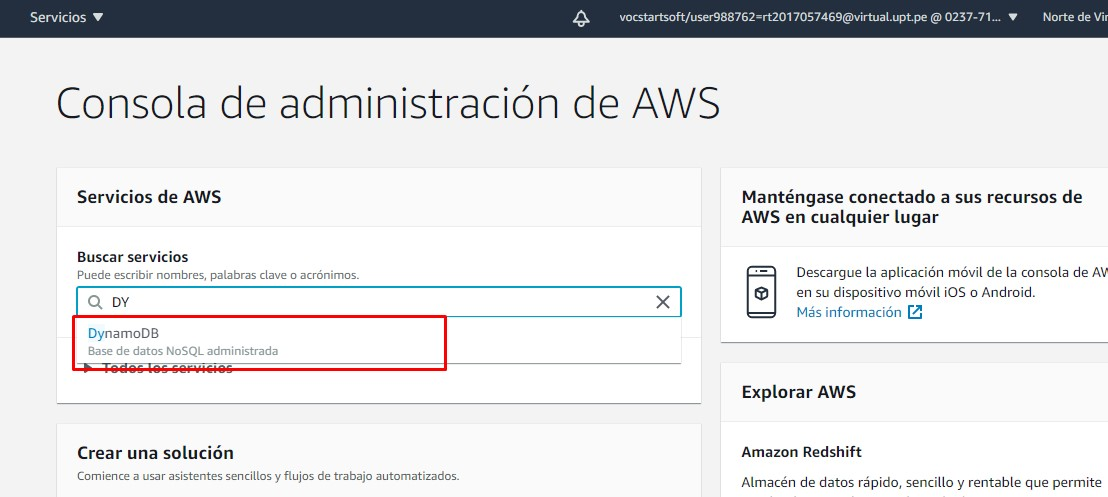
\includegraphics[width=14cm]{./img/1.jpg} 
	\end{center}
	\subsection{Paso 1: creación de una tabla NoSQL}
	
	\begin{enumerate}
		
		\item Cree un proyecto Aplicación de WPF (.NET Framework) y asígnele el nombre SimpleWPFApp.
		Se abre WPF Designer y se muestra la MainWindow del proyecto.
		\begin{center}
			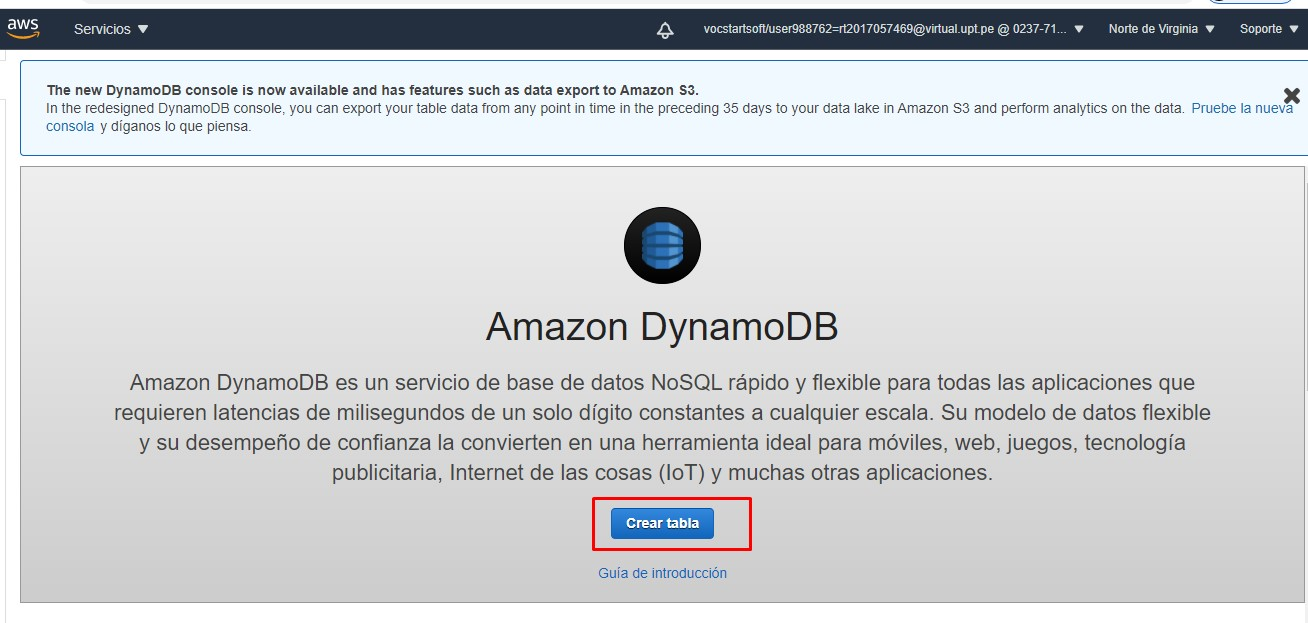
\includegraphics[width=14cm]{./img/2.jpg} 
		\end{center}
		
		\item En este tutorial utilizaremos una biblioteca de música como nuestro caso de uso.  En el campo Table name (Nombre de la tabla), escriba Music.
		\begin{center}
			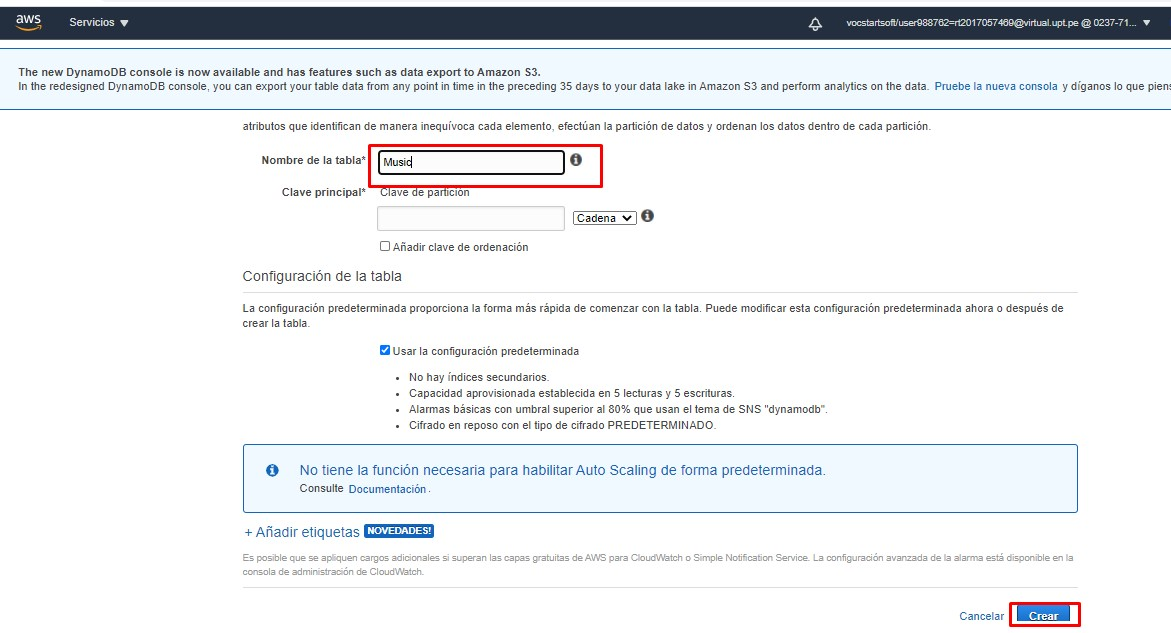
\includegraphics[width=14cm]{./img/3.jpg} 
		\end{center}
		\item  La clave de partición se utiliza para repartir datos por las particiones con fines de escalabilidad. Es importante elegir un atributo con una amplia gama de valores y que es probable que tenga patrones de acceso de distribución uniforme. Escriba Artist en el campo Partition Key (Clave de partición)..
		\begin{center}
			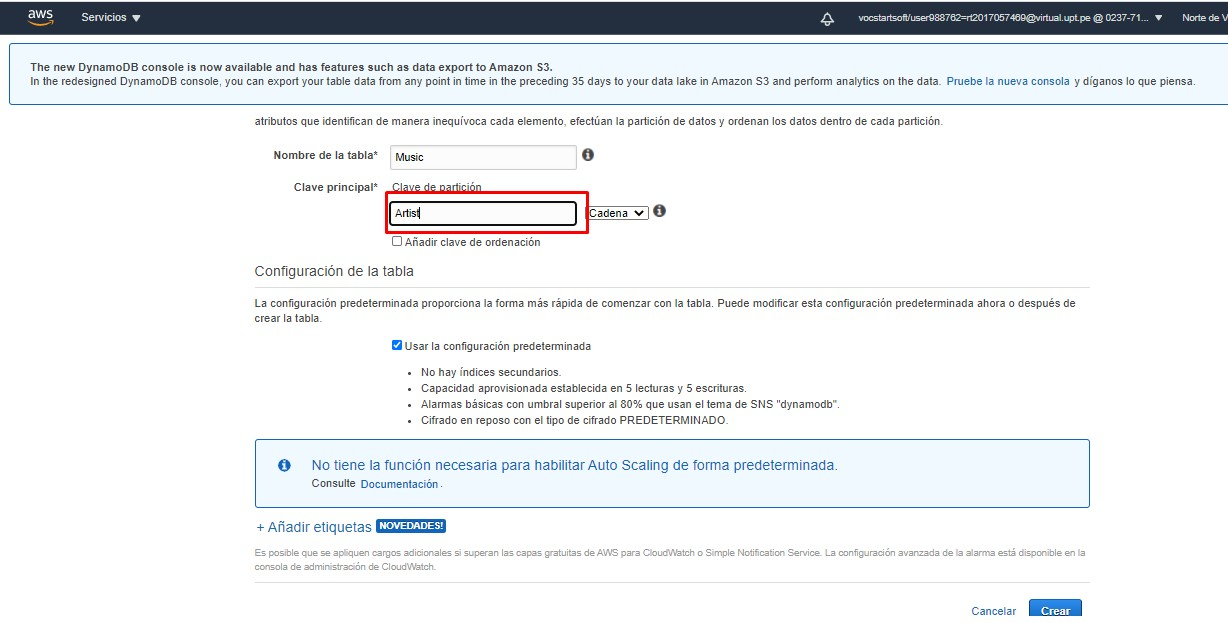
\includegraphics[width=14cm]{./img/4.jpg} 
		\end{center}
		\item Dado que cada artista puede componer muchas canciones, puede habilitar el ordenamiento sencillo con una clave de ordenamiento. Marque la casilla Add sort key (Añadir clave de ordenamiento). Escriba songTitle en el campo Add sort key (Añadir clave de ordenamiento)..
\begin{center}
	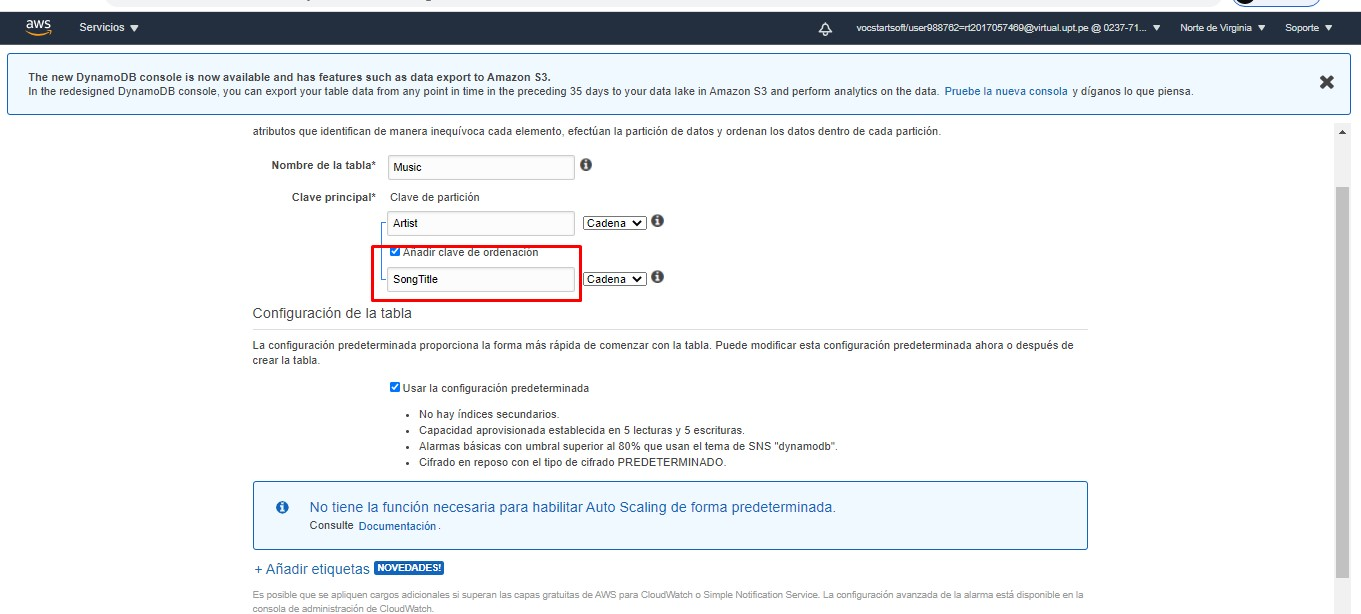
\includegraphics[width=14cm]{./img/5.jpg} 
\end{center}
		\item A continuación, activaremos DynamoDB Auto Scaling para nuestra tabla.
		
		DynamoDB Auto Scaling modificará la capacidad de lectura y escritura de su tabla en función del volumen de solicitudes. Mediante el uso de una función de AWS Identity and Access Management (IAM) denominada DynamoDBAutoscaleRole, DynamoDB administrará el proceso de Auto Scaling por usted. DynamoDB creará esta función por usted la primera vez que active Auto Scaling en una cuenta.
		
		Indique a DynamoDB que cree la función mediante la anulación de la selección de Use default settings (Utilizar configuración predeterminada).
		\begin{center}
			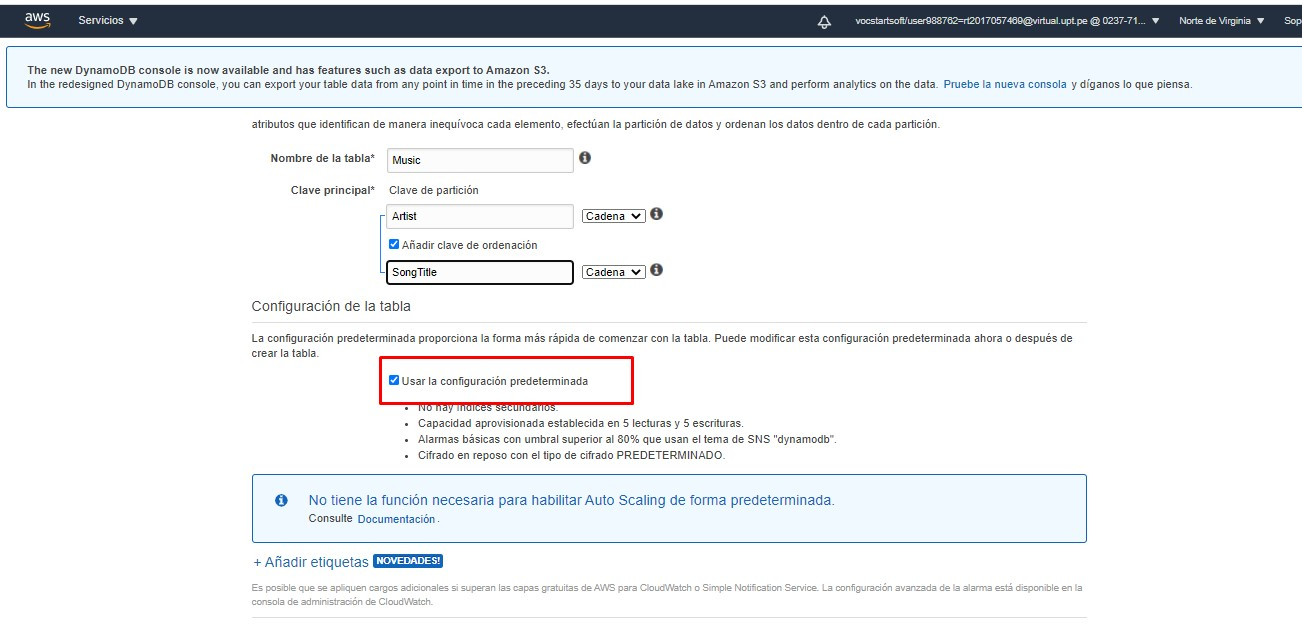
\includegraphics[width=14cm]{./img/6.jpg} 
		\end{center}
	
	\begin{center}
		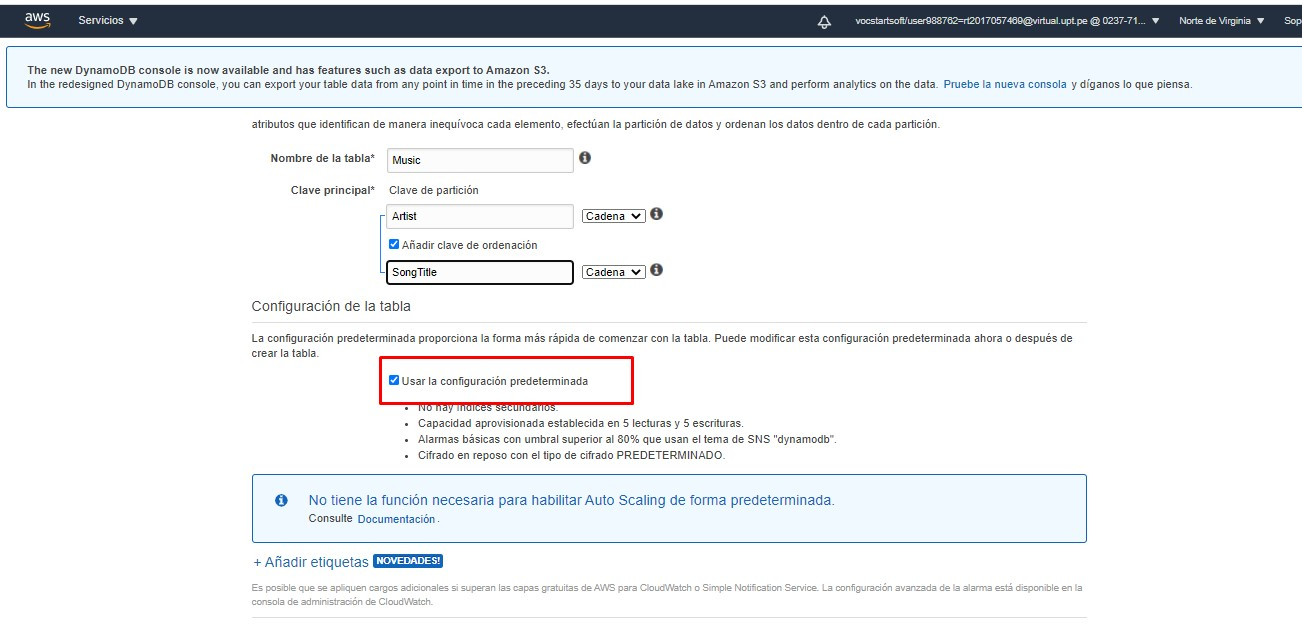
\includegraphics[width=14cm]{./img/6.jpg} 
	\end{center}
	
		\item Desplácese hacia la parte inferior de la pantalla, pasando Secondary indexes (Índices secundarios), Provisioned capacity (Capacidad aprovisionada) y Auto Scaling hasta llegar al botón Create (Crear). No modificaremos estos parámetros para los fines de este tutorial.
		
		En la sección Auto Scaling, observe que DynamoDB creará la función DynamoDBAutoscaleRole por usted.
		
		Ahora seleccione Create (Crear).
		
		Cuando la tabla Music esté lista para su uso, aparecerá en la lista de tablas con una marca de verificación .
		
		¡Enhorabuena! Acaba de crear una tabla NoSQL con la consola de DynamoDB.
		
		\begin{center}
			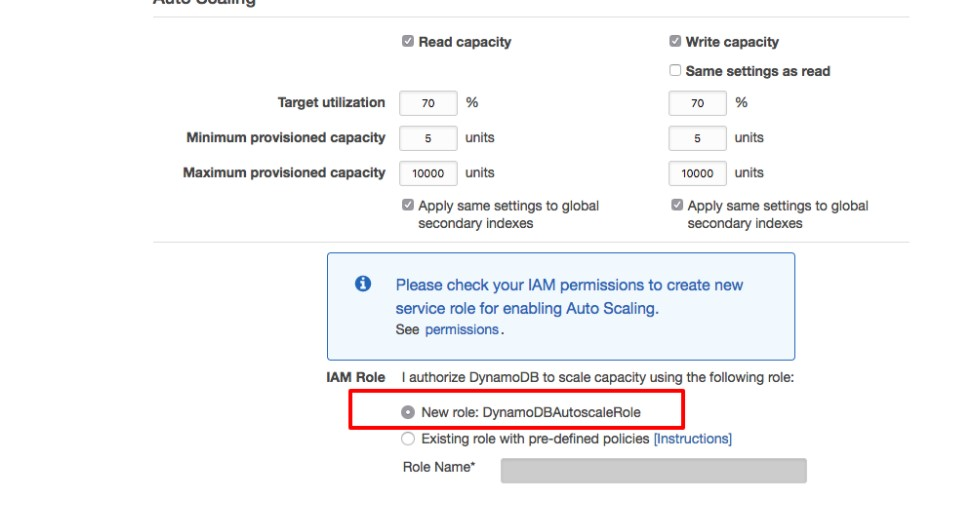
\includegraphics[width=14cm]{./img/7.jpg} 
		\end{center}
\subsection{Paso 2: agregar datos a la tabla NoSQL}
	\begin{enumerate}
		
		\item Haga clic en la pestaña Items (Elementos). Bajo la pestaña Items (Elementos), haga clic en Create item (Crear elemento) .
		\begin{center}
			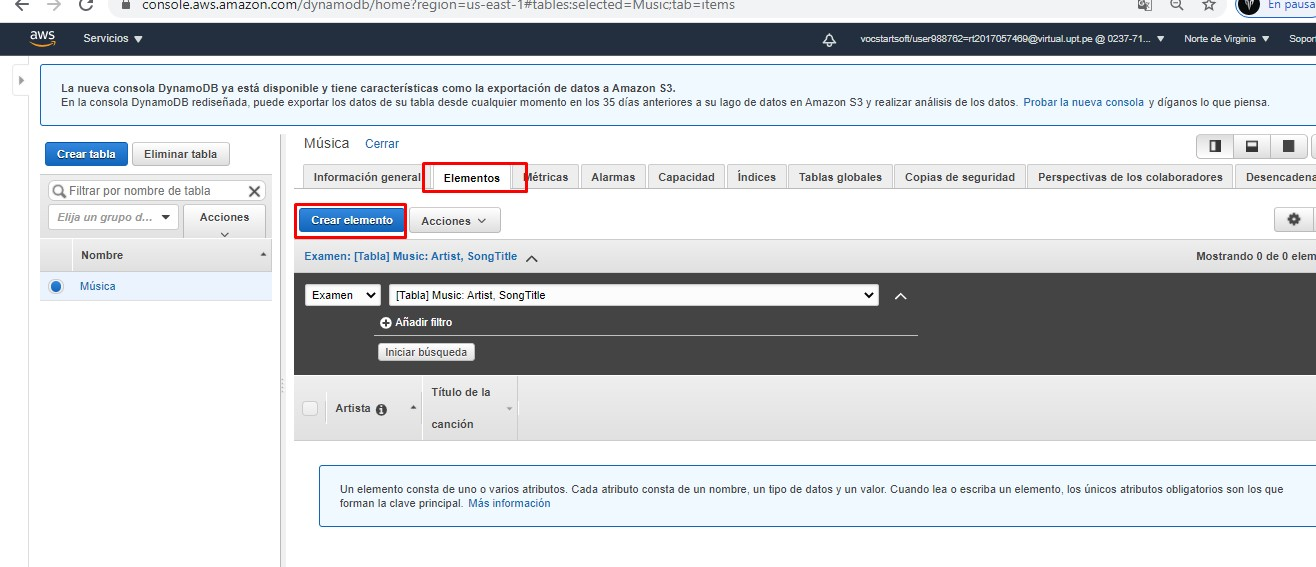
\includegraphics[width=14cm]{./img/8.jpg} 
		\end{center}
		\item En la ventana de introducción de datos, escriba lo siguiente:
		
		Para el atributo Artist, escriba No One You Know.
		Para el atributo SongTitle , escriba Call Me Today.
		Haga clic en Save (Guardar) para guardar el elemento.
		\begin{center}
			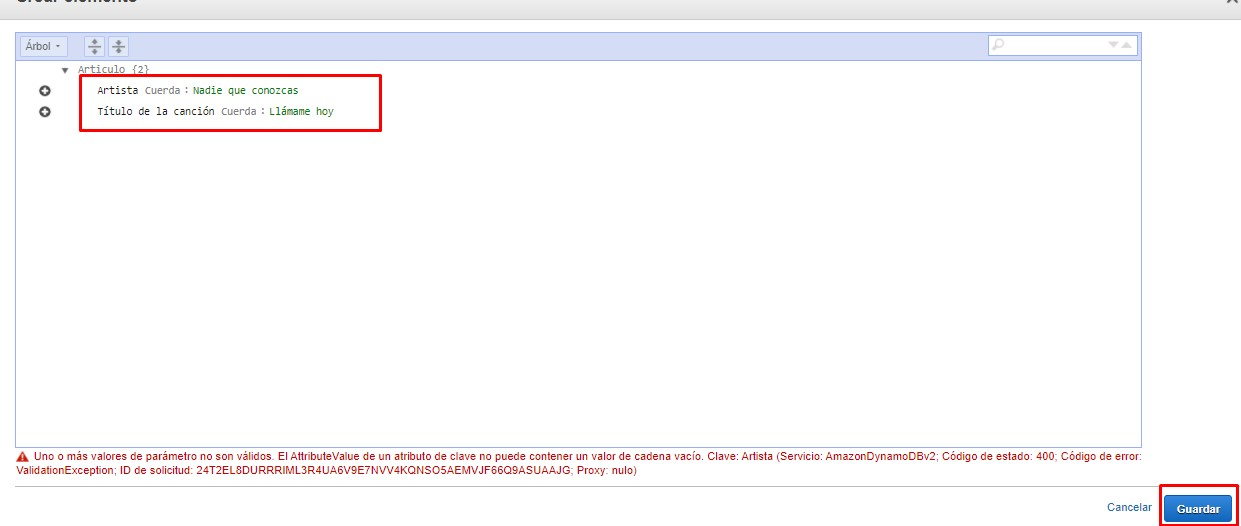
\includegraphics[width=14cm]{./img/9.jpg} 
		\end{center}
		\item Repita el proceso para agregar algunos elementos más a la tabla Music:
		
		Artist: No One You Know; songTitle: My Dog Spot
		Artist: No One You Know; songTitle: Somewhere Down The Road
		Artist: The Acme Band; songTitle: Still in Love
		Artist: The Acme Band; songTitle: Look Out, World
		\begin{center}
			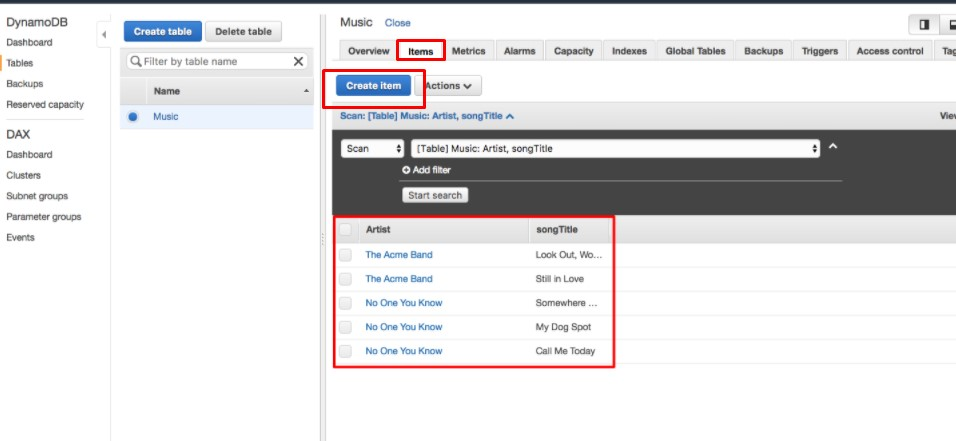
\includegraphics[width=14cm]{./img/10.jpg} 
		\end{center}
	
\end{enumerate}
	\subsection{Paso 3: consulta de la tabla NoSQL}
	\begin{enumerate}
		
		\item Mediante la lista desplegable situada en el banner gris oscuro encima de los elementos, cambie Scan (Escaneo) a Query (Consulta). 
	\begin{center}
		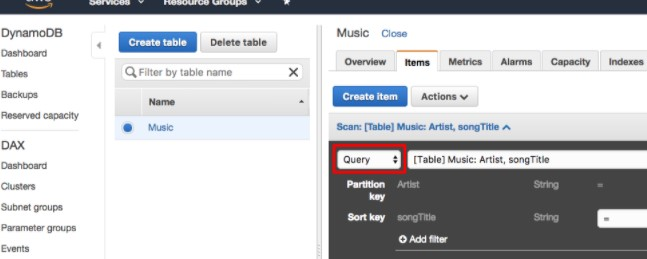
\includegraphics[width=14cm]{./img/11.jpg} 
	\end{center}
		\item Cree un acceso directo en el escritorio a la aplicación SimpleWPFApp. Haga clic con el botón derecho
		en SimpleWPFApp.exe y elija Copiar. En el escritorio, haga clic con el botón derecho y elija Pegar
		acceso directo.
		Sugerencia
		Un acceso directo a la aplicación facilita el poder agregar o modificar pruebas automatizadas de IU
		para la aplicación porque permite iniciar la aplicación rápidamente.
		\begin{center}
			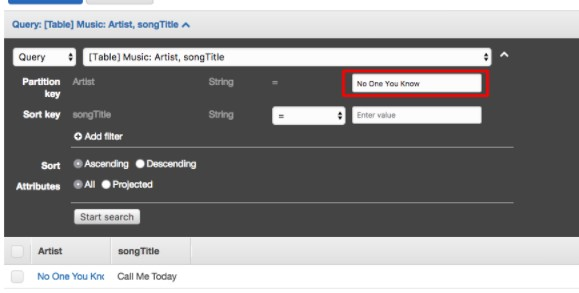
\includegraphics[width=14cm]{./img/12.jpg} 
		\end{center}
		\item
		 Pruebe con otra consulta, pero esta vez acote los resultados de búsqueda:
		
		En el campo Artist, escriba The Acme Band.
		En el campo SongTitle, seleccione Begins with (Empieza por) en la lista desplegable y escriba S.
		Haga clic en Start search (Iniciar búsqueda).  Solo se muestra “Still in Love” interpretada por The Acme Band.
		\begin{center}
			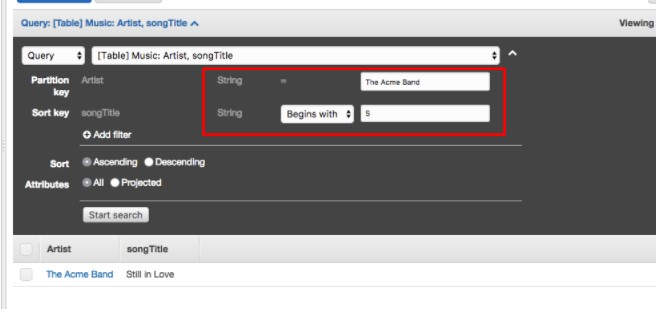
\includegraphics[width=14cm]{./img/13.jpg} 
		\end{center}
\end{enumerate}	
	\subsection{Paso 4: eliminación de un elemento existente}
	\begin{enumerate}
		
		\item En el Explorador de soluciones, haga clic con el botón derecho en la solución y
		elija Agregar > Nuevo proyecto
		\begin{center}
			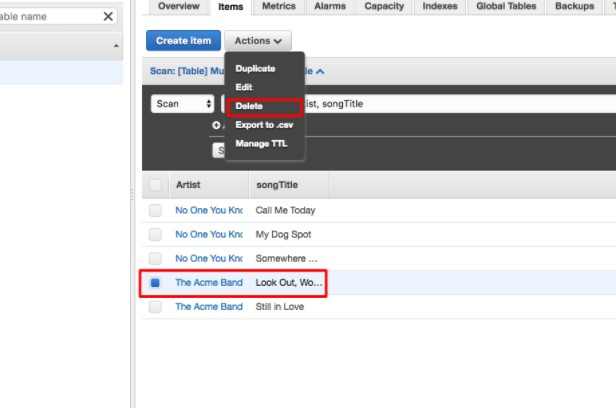
\includegraphics[width=14cm]{./img/14.jpg} 
		\end{center}
		
		
	
\end{enumerate}	
	\subsection{Paso 5: eliminación de una tabla NoSQL}
	\begin{enumerate}
		
		\item Puede eliminar con facilidad una tabla de la consola Amazon DynamoDB. Se recomienda eliminar las tablas que ya no utilice para que no le sigan cobrando por ellas.
		\\
		En la consola de DynamoDB, haga clic en el botón de selección ubicado junto a la tabla Music y, a continuación, haga clic en Delete table (Eliminar tabla).
		En el cuadro de diálogo de confirmación, haga clic en Delete (Eliminar).
\begin{center}
	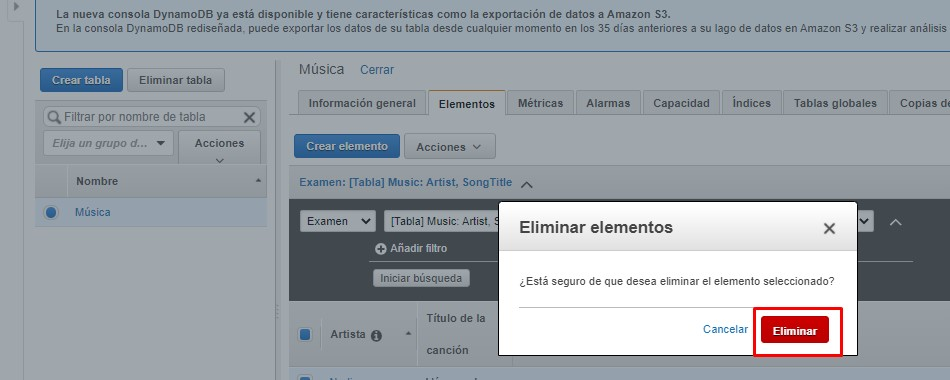
\includegraphics[width=14cm]{./img/15.jpg} 
\end{center}
		
		
		
	\section{CONCLUSIONES}
	\begin{itemize}
			\item Se realizo con exito la creacion de tablas y agregacion de datos
			\\
			Se analizo realizando consultas de datos y finalmente se elimino la tabla
		\end{itemize}
		
		
	\end{enumerate}